\section{Results}\label{sec:results}

All results use LightGBM as base model and nominal level 0.90, unless stated otherwise. A negative CE contrast means that the first method is better calibrated. The exploratory results carry no confirmatory claim. The word ``significant'' is not used for any result outside the pre-specified family, and unadjusted $p$-values are given as descriptive. Sections~\ref{sec:explor} to~\ref{sec:width} concern the design panel and the first hold-out panel; Section~\ref{sec:panel2} reports the extension (second hold-out panel, four base models) and is kept apart because the panel, the base models and the start date differ; Section~\ref{sec:ablation} collects the ablation analyses (base model, warm-up, feedback delay, native intervals and Chronos accuracy).

\subsection{Calibration of adaptive methods against the baselines}\label{sec:explor}

Figure~\ref{fig:coverage_h} shows pooled coverage by method and horizon for the panels of the study, and Figure~\ref{fig:ce_bars} the calibration error. The exploratory run covers 13 units, origins from 2000-01 and target months to 2025-06, with warm-up 48. Pooled coverage at $h=1,3,6,12$ is 0.946, 0.937, 0.917 and 0.864 for split conformal; 0.917, 0.916, 0.900 and 0.869 for rolling; and 0.908, 0.906, 0.899 and 0.864 for ACI (the number of unit-months is 2024, 1972, 1894 and 1738; the full table is in Appendix~\ref{app:extra}). Split conformal over-covers at short horizons, so that a lower coverage there is closer to nominal. Bootstrap 95 percent intervals are wide: for ACI they are \ci{0.879}{0.930} at $h=3$ and \ci{0.797}{0.914} at $h=12$.

\begin{figure}[t]
\centering
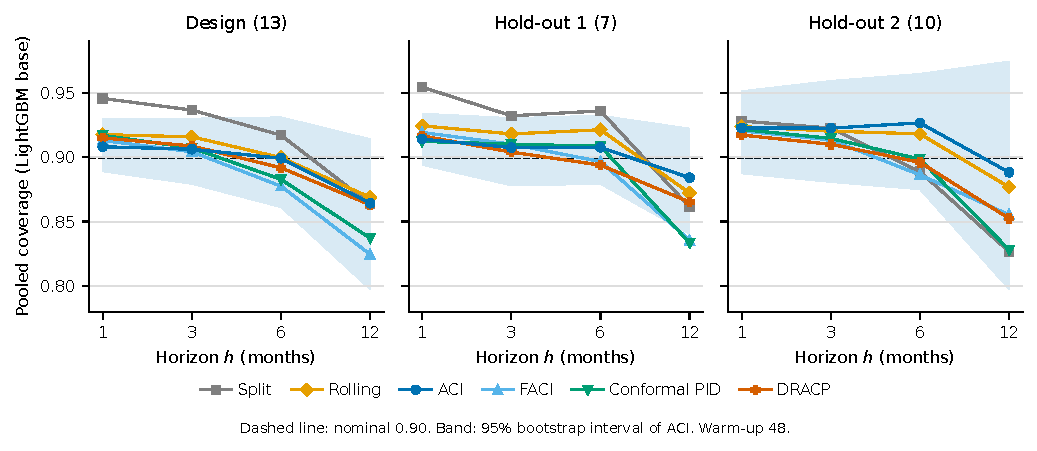
\includegraphics[width=\linewidth]{figures/fig_coverage_h.pdf}
\caption{Pooled empirical coverage by horizon and interval method for each panel (LightGBM base), against the nominal level 0.90.}
\label{fig:coverage_h}
\end{figure}

\begin{figure}[t]
\centering
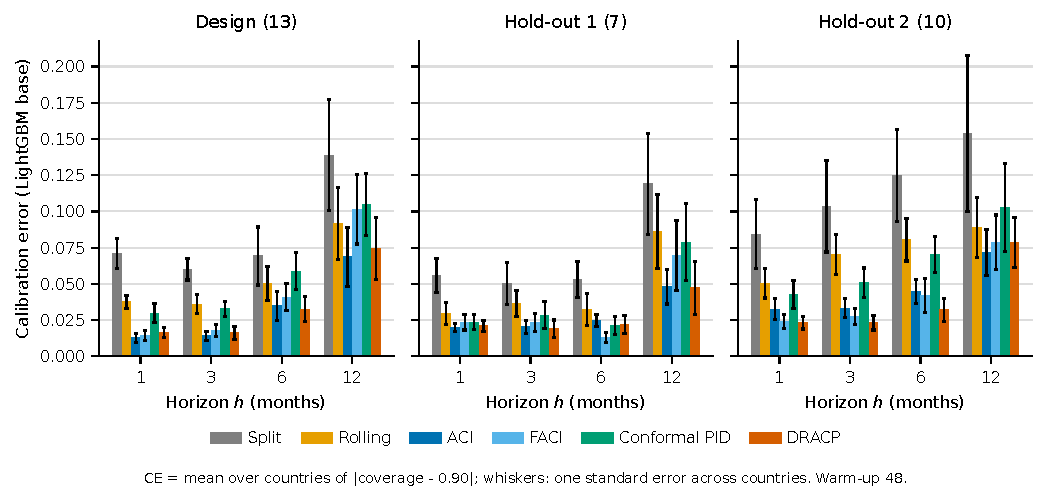
\includegraphics[width=\linewidth]{figures/fig_ce_bars.pdf}
\caption{Calibration error (mean over countries of $|\text{coverage}-0.90|$) by interval method and horizon for each panel (LightGBM base).}
\label{fig:ce_bars}
\end{figure}

Tables~\ref{tab:ce_expl} and~\ref{tab:ce_ho1} give the calibration error on the design panel and on the first hold-out panel. In the exploratory data the CE of ACI at $h=1,3,6,12$ is 0.013, 0.014, 0.035 and 0.069, against 0.038, 0.036, 0.050 and 0.091 for rolling and 0.071, 0.060, 0.069 and 0.139 for split. On the first hold-out panel it is 0.020, 0.020, 0.025 and 0.048 for ACI, 0.029, 0.036, 0.032 and 0.086 for rolling, and 0.056, 0.050, 0.053 and 0.119 for split; DRACP has 0.021, 0.019, 0.022 and 0.047, FACI 0.024, 0.023, 0.013 and 0.070, and conformal PID 0.024, 0.028, 0.021 and 0.079.

\begin{table}[t]
\centering
\caption{Calibration error by base model, interval method and horizon, design panel (13 countries, exploratory, warm-up 48).}
\label{tab:ce_expl}
\small
\fittable{\begin{tabular}{llrrrr}
\toprule
Base model & Interval & $h{=}1$ & $h{=}3$ & $h{=}6$ & $h{=}12$ \\
\midrule
LightGBM & Split & 0.071 & 0.060 & 0.069 & 0.139 \\
 & Rolling & 0.038 & 0.036 & 0.050 & 0.091 \\
 & ACI & 0.013 & 0.014 & 0.035 & 0.069 \\
 & FACI & 0.014 & 0.018 & 0.041 & 0.101 \\
 & Conformal PID & 0.030 & 0.033 & 0.059 & 0.105 \\
 & DRACP & 0.016 & 0.016 & 0.033 & 0.074 \\
\midrule
ARIMA & Split & 0.064 & 0.064 & 0.098 & 0.148 \\
 & Rolling & 0.031 & 0.032 & 0.058 & 0.096 \\
 & ACI & 0.010 & 0.015 & 0.026 & 0.079 \\
 & FACI & 0.017 & 0.023 & 0.029 & 0.102 \\
 & Conformal PID & 0.027 & 0.020 & 0.046 & 0.099 \\
 & DRACP & 0.012 & 0.015 & 0.021 & 0.072 \\
 & Native & 0.047 & 0.066 & 0.089 & 0.137 \\
\midrule
Naive B & Split & 0.057 & 0.069 & 0.073 & 0.171 \\
 & Rolling & 0.031 & 0.035 & 0.043 & 0.100 \\
 & ACI & 0.012 & 0.016 & 0.024 & 0.057 \\
 & FACI & 0.017 & 0.018 & 0.039 & 0.124 \\
 & Conformal PID & 0.025 & 0.021 & 0.036 & 0.113 \\
 & DRACP & 0.017 & 0.017 & 0.028 & 0.071 \\
\midrule
ETS & Native & 0.044 & 0.051 & 0.064 & 0.116 \\
\bottomrule
\end{tabular}
}
\end{table}

\begin{table}[t]
\centering
\caption{Calibration error by base model, interval method and horizon, first hold-out panel (7 countries, warm-up 48).}
\label{tab:ce_ho1}
\small
\fittable{\begin{tabular}{llrrrr}
\toprule
Base model & Interval & $h{=}1$ & $h{=}3$ & $h{=}6$ & $h{=}12$ \\
\midrule
LightGBM & Split & 0.056 & 0.050 & 0.053 & 0.119 \\
 & Rolling & 0.029 & 0.036 & 0.032 & 0.086 \\
 & ACI & 0.020 & 0.020 & 0.025 & 0.048 \\
 & FACI & 0.023 & 0.023 & 0.013 & 0.070 \\
 & Conformal PID & 0.024 & 0.028 & 0.021 & 0.079 \\
 & DRACP & 0.021 & 0.019 & 0.022 & 0.047 \\
\midrule
ARIMA & Split & 0.067 & 0.065 & 0.061 & 0.106 \\
 & Rolling & 0.039 & 0.043 & 0.040 & 0.069 \\
 & ACI & 0.014 & 0.013 & 0.024 & 0.040 \\
 & FACI & 0.019 & 0.010 & 0.029 & 0.084 \\
 & Conformal PID & 0.029 & 0.037 & 0.034 & 0.083 \\
 & DRACP & 0.020 & 0.011 & 0.027 & 0.051 \\
 & Native & 0.053 & 0.058 & 0.062 & 0.073 \\
\midrule
Naive B & Split & 0.063 & 0.049 & 0.135 & 0.175 \\
 & Rolling & 0.039 & 0.030 & 0.061 & 0.052 \\
 & ACI & 0.015 & 0.021 & 0.030 & 0.032 \\
 & FACI & 0.026 & 0.020 & 0.036 & 0.079 \\
 & Conformal PID & 0.030 & 0.027 & 0.050 & 0.070 \\
 & DRACP & 0.024 & 0.024 & 0.032 & 0.055 \\
\midrule
ETS & Native & 0.056 & 0.035 & 0.048 & 0.053 \\
\bottomrule
\end{tabular}
}
\end{table}

The exploratory contrasts of the primary family are, at warm-up 48, ACI minus rolling $-2.2$~pp at $h=3$ and $-1.5$~pp at $h=6$ with unadjusted $p$-values 0.030 and 0.020 but Holm-adjusted 0.090 and 0.078, so neither survives the correction for the family. ACI minus split (secondary) was $-4.6$~pp at $h=3$ (95\% interval \ci{-5.0}{-1.4}, unadjusted $p=0.001$) and $-3.4$~pp at $h=6$ ($p=0.0025$). DRACP minus ACI was $+0.2$~pp and $-0.2$~pp, within noise. Equivalence within 2~pp was shown at warm-up 48 (maximum one-sided $p$ 0.0085 at $h=3$ and 0.0135 at $h=6$) and not shown at warm-up 96 (0.128 and 0.146). At warm-up 96, in the exploratory data, DRACP was wider than ACI: its Winkler score was higher by 33.2 percent at $h=3$ (95\% interval \ci{12.1}{75.9}, unadjusted $p=0.049$) and 19.9 percent at $h=6$ (\ci{6.8}{46.2}, $p=0.054$). Equivalence in the exploratory data is therefore not stable across warm-up sizes.

Further exploratory observations. At $h=3$ split coverage ranges from 0.822 (Peru) and 0.827 (Kazakhstan) to 1.000 (Indonesia), while ACI ranges from 0.886 to 0.934 (Figure~\ref{fig:country_cov}); at $h=12$ ACI coverage ranges from 0.655 (Peru) and 0.716 (Nigeria) to 1.000 (Uzbekistan). At $h=12$ pooled coverage is below nominal for every method (0.825 to 0.869) and the adaptive methods do not repair it; the bootstrap interval of ACI, \ci{0.797}{0.914}, includes 0.90, and so do those of DRACP, rolling and split (upper limits 0.918, 0.920 and 0.915), but those of FACI and conformal PID do not (0.876 and 0.897). Mean absolute error relative to naive B was 0.74 (ARIMA), 0.72 (ETS) and 0.74 (LightGBM) at $h=3$, 0.75, 0.76 and 0.75 at $h=6$, and 0.86, 0.93 and 0.91 at $h=12$.

\subsection{First hold-out panel and the decision rules R1--R5}\label{sec:holdout}

The hold-out run covers 7 countries, target months 2009-02 to 2026-06, with 205 and 199 pooled months at $h=3$ and $h=6$ for run A (warm-up 48) and 157 and 151 for run B (warm-up 96); the number of unit-months in run A is 1163, 1135, 1093 and 1009 at $h=1,3,6,12$. Pooled coverage in run A at $h=1,3,6,12$ is 0.954, 0.932, 0.936 and 0.861 for split, 0.924, 0.918, 0.921 and 0.872 for rolling, 0.914, 0.907, 0.908 and 0.884 for ACI, 0.919, 0.910, 0.897 and 0.835 for FACI, 0.912, 0.910, 0.909 and 0.833 for conformal PID, and 0.917, 0.904, 0.894 and 0.865 for DRACP (Appendix~\ref{app:extra}). At $h=12$ the pooled coverage of every method is below 0.90 (0.833 to 0.884); the bootstrap upper limits for ACI, DRACP, rolling and split (0.923, 0.901, 0.918 and 0.919) do not exclude 0.90, those of FACI and conformal PID (0.885 and 0.884) do. Table~\ref{tab:contrasts} gives the calibration-error contrasts and Table~\ref{tab:tost} the equivalence tests; the decision rules are applied as pre-specified.

\begin{table}[t]
\centering
\caption{Primary-family calibration-error contrasts by panel and base model: $T$ (pp of CE), 95\% block-bootstrap interval, Holm-adjusted $p$, minimum detectable difference (MDE) and verdict under the power rule.}
\label{tab:contrasts}
\small
\fittable{\begin{tabular}{llcllrrrl}
\toprule
Panel & Base & $h$ & Contrast & $T$ (pp) & 95\% CI & Holm $p$ & MDE (pp) & Verdict \\
\midrule
Design (13) & LightGBM & 3 & ACI $-$ rolling & $-$2.2 & [$-$2.7, +0.1] & 0.090 & -- & Inconclusive \\
 &  & 6 & ACI $-$ rolling & $-$1.5 & [$-$2.1, $-$0.1] & 0.078 & -- & Inconclusive \\
 &  & 3 & DRACP $-$ ACI & +0.2 & [$-$1.2, +1.0] & 1.000 & -- & Inconclusive \\
 &  & 6 & DRACP $-$ ACI & $-$0.2 & [$-$2.0, +1.3] & 1.000 & -- & Inconclusive \\
\midrule
Hold-out 1 (7) & LightGBM & 3 & ACI $-$ rolling & $-$1.6 & [$-$3.0, +0.5] & 0.350 & -- & Inconclusive \\
 &  & 6 & ACI $-$ rolling & $-$0.7 & [$-$2.8, +1.3] & 1.000 & -- & Inconclusive \\
 &  & 3 & DRACP $-$ ACI & $-$0.1 & [$-$1.2, +0.9] & 1.000 & -- & Inconclusive \\
 &  & 6 & DRACP $-$ ACI & $-$0.3 & [$-$1.4, +1.7] & 1.000 & -- & Inconclusive \\
\midrule
Design (13), from 2010 & LightGBM & 3 & ACI $-$ rolling & $-$2.1 & [$-$2.9, +0.5] & 0.216 & -- & Inconclusive \\
 &  & 6 & ACI $-$ rolling & $-$2.0 & [$-$3.1, +0.5] & 0.216 & -- & Inconclusive \\
 &  & 3 & DRACP $-$ ACI & $-$0.5 & [$-$1.6, +1.3] & 0.654 & -- & Inconclusive \\
 &  & 6 & DRACP $-$ ACI & +1.9 & [$-$1.0, +5.5] & 0.654 & -- & Inconclusive \\
\midrule
Design (13), from 2010 & Chronos & 3 & ACI $-$ rolling & $-$1.9 & [$-$2.3, +0.9] & 0.363 & -- & Inconclusive \\
 &  & 6 & ACI $-$ rolling & $-$2.0 & [$-$2.5, +0.8] & 0.358 & -- & Inconclusive \\
 &  & 3 & DRACP $-$ ACI & +0.0 & [$-$1.4, +1.3] & 0.982 & -- & Inconclusive \\
 &  & 6 & DRACP $-$ ACI & +2.4 & [$-$0.6, +5.9] & 0.363 & -- & Inconclusive \\
\midrule
Hold-out 1 (7), from 2010 & LightGBM & 3 & ACI $-$ rolling & $-$2.4 & [$-$5.5, +0.7] & 0.496 & -- & Inconclusive \\
 &  & 6 & ACI $-$ rolling & $-$4.7 & [$-$9.6, +0.5] & 0.390 & -- & Inconclusive \\
 &  & 3 & DRACP $-$ ACI & $-$0.8 & [$-$2.2, +1.2] & 0.656 & -- & Inconclusive \\
 &  & 6 & DRACP $-$ ACI & +0.2 & [$-$2.2, +1.4] & 0.904 & -- & Inconclusive \\
\midrule
Hold-out 1 (7), from 2010 & Chronos & 3 & ACI $-$ rolling & $-$1.3 & [$-$4.9, +0.7] & 1.000 & -- & Inconclusive \\
 &  & 6 & ACI $-$ rolling & $-$2.0 & [$-$4.5, +1.4] & 0.962 & -- & Inconclusive \\
 &  & 3 & DRACP $-$ ACI & $-$0.2 & [$-$2.0, +1.2] & 1.000 & -- & Inconclusive \\
 &  & 6 & DRACP $-$ ACI & +0.2 & [$-$2.5, +4.3] & 1.000 & -- & Inconclusive \\
\midrule
Hold-out 2 (10) & LightGBM & 3 & ACI $-$ rolling & $-$3.7 & [$-$5.1, $-$0.7] & 0.008 & 3.2 & Met \\
 &  & 6 & ACI $-$ rolling & $-$3.5 & [$-$4.9, +0.5] & 0.159 & 6.1 & Not met \\
 &  & 3 & DRACP $-$ ACI & $-$1.0 & [$-$2.0, +0.9] & 0.321 & -- & Inconclusive \\
 &  & 6 & DRACP $-$ ACI & $-$1.3 & [$-$2.7, +2.0] & 0.337 & -- & Inconclusive \\
\midrule
Hold-out 2 (10) & ARIMA & 3 & ACI $-$ rolling & $-$3.2 & [$-$3.6, $-$1.1] & 0.004 & 3.2 & Met \\
 &  & 6 & ACI $-$ rolling & $-$3.1 & [$-$3.9, $-$0.5] & 0.030 & 3.5 & Met \\
 &  & 3 & DRACP $-$ ACI & $-$1.5 & [$-$2.4, +0.8] & 0.199 & -- & Inconclusive \\
 &  & 6 & DRACP $-$ ACI & $-$1.8 & [$-$3.4, +0.7] & 0.199 & -- & Inconclusive \\
\midrule
Hold-out 2 (10) & Naive B & 3 & ACI $-$ rolling & $-$4.1 & [$-$4.9, $-$1.5] & 0.004 & 1.2 & Met \\
 &  & 6 & ACI $-$ rolling & $-$3.4 & [$-$4.7, $-$0.4] & 0.039 & 3.5 & Met \\
 &  & 3 & DRACP $-$ ACI & $-$1.2 & [$-$2.3, +0.9] & 0.422 & -- & Inconclusive \\
 &  & 6 & DRACP $-$ ACI & $-$1.8 & [$-$3.3, +2.5] & 0.422 & -- & Inconclusive \\
\midrule
Hold-out 2 (10) & Chronos & 3 & ACI $-$ rolling & $-$3.3 & [$-$4.0, $-$0.3] & 0.036 & -- & Inconclusive \\
 &  & 6 & ACI $-$ rolling & $-$2.5 & [$-$3.6, +0.1] & 0.088 & 6.6 & Not met \\
 &  & 3 & DRACP $-$ ACI & $-$0.5 & [$-$1.8, +1.3] & 0.454 & -- & Inconclusive \\
 &  & 6 & DRACP $-$ ACI & $-$1.2 & [$-$2.2, +1.3] & 0.443 & -- & Inconclusive \\
\bottomrule
\end{tabular}
}
\end{table}

\begin{table}[t]
\centering
\caption{Equivalence of DRACP and ACI by two one-sided tests with a margin of 2~pp of CE, and the status of each contrast under the power rule.}
\label{tab:tost}
\small
\fittable{\begin{tabular}{lcclrrll}
\toprule
Panel & Warm-up & Base & $h$ & $T$ (pp) & TOST $p$ & TOST verdict & Under E5 \\
\midrule
Design (13) & 48 & LightGBM & 3 & +0.2 & 0.008 & Equivalent & Inconclusive \\
 &  &  & 6 & $-$0.2 & 0.013 & Equivalent & Inconclusive \\
\midrule
Design (13) & 96 & LightGBM & 3 & +0.1 & 0.128 & Not shown & Not assessed \\
 &  &  & 6 & +0.2 & 0.146 & Not shown & Not assessed \\
\midrule
Hold-out 1 (7) & 48 & LightGBM & 3 & $-$0.1 & $<$0.001 & Equivalent & Inconclusive \\
 &  &  & 6 & $-$0.3 & 0.047 & Equivalent & Inconclusive \\
\midrule
Hold-out 1 (7) & 96 & LightGBM & 3 & $-$0.4 & 0.062 & Not shown & Inconclusive \\
 &  &  & 6 & $-$1.1 & 0.355 & Not shown & Inconclusive \\
\midrule
Design (13), from 2010 & 48 & LightGBM & 3 & $-$0.5 & 0.070 & Not shown & Inconclusive \\
 &  &  & 6 & +1.9 & 0.452 & Not shown & Inconclusive \\
 & 48 & Chronos & 3 & +0.0 & 0.004 & Equivalent & Inconclusive \\
 &  &  & 6 & +2.4 & 0.520 & Not shown & Inconclusive \\
\midrule
Hold-out 1 (7), from 2010 & 48 & LightGBM & 3 & $-$0.8 & 0.124 & Not shown & Inconclusive \\
 &  &  & 6 & +0.2 & 0.080 & Not shown & Inconclusive \\
 & 48 & Chronos & 3 & $-$0.2 & 0.016 & Equivalent & Inconclusive \\
 &  &  & 6 & +0.2 & 0.134 & Not shown & Inconclusive \\
\midrule
Hold-out 2 (10) & 48 & LightGBM & 3 & $-$1.0 & 0.153 & Not shown & Inconclusive \\
 &  &  & 6 & $-$1.3 & 0.472 & Not shown & Inconclusive \\
 & 48 & ARIMA & 3 & $-$1.5 & 0.379 & Not shown & Inconclusive \\
 &  &  & 6 & $-$1.8 & 0.553 & Not shown & Inconclusive \\
 & 48 & Naive B & 3 & $-$1.2 & 0.352 & Not shown & Inconclusive \\
 &  &  & 6 & $-$1.8 & 0.760 & Not shown & Inconclusive \\
 & 48 & Chronos & 3 & $-$0.5 & 0.038 & Equivalent & Inconclusive \\
 &  &  & 6 & $-$1.2 & 0.372 & Not shown & Inconclusive \\
\midrule
Hold-out 2 (10) & 96 & LightGBM & 3 & $-$0.5 & 0.037 & Equivalent & Inconclusive \\
 &  &  & 6 & $-$3.0 & 0.982 & Not shown & Inconclusive \\
 & 96 & ARIMA & 3 & +0.3 & 0.300 & Not shown & Inconclusive \\
 &  &  & 6 & $-$2.3 & 0.787 & Not shown & Inconclusive \\
 & 96 & Naive B & 3 & $-$0.2 & 0.013 & Equivalent & Inconclusive \\
 &  &  & 6 & $-$2.3 & 0.868 & Not shown & Inconclusive \\
 & 96 & Chronos & 3 & $-$1.2 & 0.189 & Not shown & Inconclusive \\
 &  &  & 6 & $-$3.0 & 0.971 & Not shown & Inconclusive \\
\bottomrule
\end{tabular}
}
\end{table}

\paragraph{R1 (ACI better calibrated than split): not met in the primary run; met at warm-up 96, which is a sensitivity run and is not promoted.} At warm-up 48 the CE difference ACI minus split was $-3.0$~pp ($p=0.054$) at $h=3$ and $-2.8$~pp ($p=0.092$) at $h=6$, with confidence intervals \ci{-5.4}{+0.5} and \ci{-3.9}{+1.2} that include zero. At warm-up 96 it was $-4.1$~pp ($p=0.018$) and $-5.9$~pp ($p=0.0025$). The direction replicates in both runs. The $p$-values for this secondary contrast are unadjusted bootstrap $p$-values; the result files have no Holm column for it, although R1 is written in terms of Holm $p$. Applying Holm over the two horizons gives 0.108 at both horizons at warm-up 48 and 0.018 ($h=3$) and 0.005 ($h=6$) at warm-up 96. At warm-up 48 the rule fails with unadjusted $p$-values as well as with Holm-adjusted ones. The pre-specified verdict is ``not met'' for the primary configuration, and warm-up 96 was not promoted to the primary configuration because R1 holds there.

\paragraph{R2 (ACI improves on rolling): not shown on this panel (MDE undefined, inconclusive).} Holm $p$ was 0.35 ($h=3$) and 1.0 ($h=6$) at warm-up 48, and 0.59 and 0.99 at warm-up 96; the point estimates are $-1.6$ and $-0.7$~pp at warm-up 48. On the Winkler score, ACI was 1.0 percent lower than rolling at $h=3$ (95\% interval \ci{-7.1}{+4.1}) and 5.3 percent higher at $h=6$ (\ci{+1.4}{+8.1}, unadjusted $p=0.005$; at warm-up 96, $+9.2$ percent, \ci{3.4}{15.3}, unadjusted $p=0.001$). These Winkler contrasts are descriptive and unadjusted. On the second hold-out panel the same rule is met at warm-up 48 in several cells; the two results are not combined (Section~\ref{sec:panel2}).

\paragraph{R3 (DRACP against ACI): inconclusive.} Equivalence within 2~pp was shown at warm-up 48 (TOST $p$ 0.0005 at $h=3$ and 0.047 at $h=6$) and not shown at warm-up 96 (0.062 and 0.355). The registered wording ``no advantage, equivalent within 2~pp'' requires equivalence at both warm-ups, so the verdict is ``inconclusive'' and the equivalence result is not stable. DRACP minus ACI is not negative with Holm $p$ below 0.05 at either warm-up, so ``DRACP better'' is also not supported. The wording used for DRACP is therefore: no advantage over ACI was detected in this configuration; equivalence within 2~pp held at warm-up 48 but not at 96. The 2~pp margin is of the size of the calibration error of ACI itself (Section~\ref{sec:discussion}), so even the equivalence verdict at warm-up 48 is weak.

\paragraph{R4 (delayed feedback explains the $h=12$ shortfall; ACI at least $+3$~pp): not met.} ACI coverage at $h=12$ was 0.884 with delayed feedback and 0.908 with instant feedback, a difference of $+2.4$~pp (Section~\ref{sec:feedback}).

\paragraph{R5 (power): all four primary contrasts are inconclusive.} The minimum detectable difference is undefined on the full hold-out sample at both warm-ups: the baseline calibration error is too small for a 10~pp improvement to be attainable, so the power at 10~pp is below 0.80. On random 15-month windows of the hold-out data the median MDE is 2.6 to 3.1~pp, but 63 to 68 percent of windows have an undefined MDE. The full-sample MDE is also undefined in the exploratory data at warm-up 48. Under R5, a contrast with an undefined MDE is inconclusive regardless of its $p$-value, so none of the four primary contrasts supports a conclusion.

Table~\ref{tab:rules} lists the five rules with their recorded outcomes.

\paragraph{What the hold-out result supports.} Adaptive methods are better calibrated than a one-shot conformal calibration, with a direction replicated in the exploratory data and in the hold-out data at both warm-up sizes and a strength of evidence that depends on the warm-up; at the primary warm-up the confidence intervals include zero. On this panel the result does not support the statements that adaptivity helps beyond a simple rolling window, or that DRACP is better than ACI. Per-country coverage varies widely: at $h=12$ the standard deviation of coverage across units is 0.058 for ACI and 0.152 for split; Figure~\ref{fig:country_cov} shows the per-country coverage of ACI.

\begin{figure}[t]
\centering
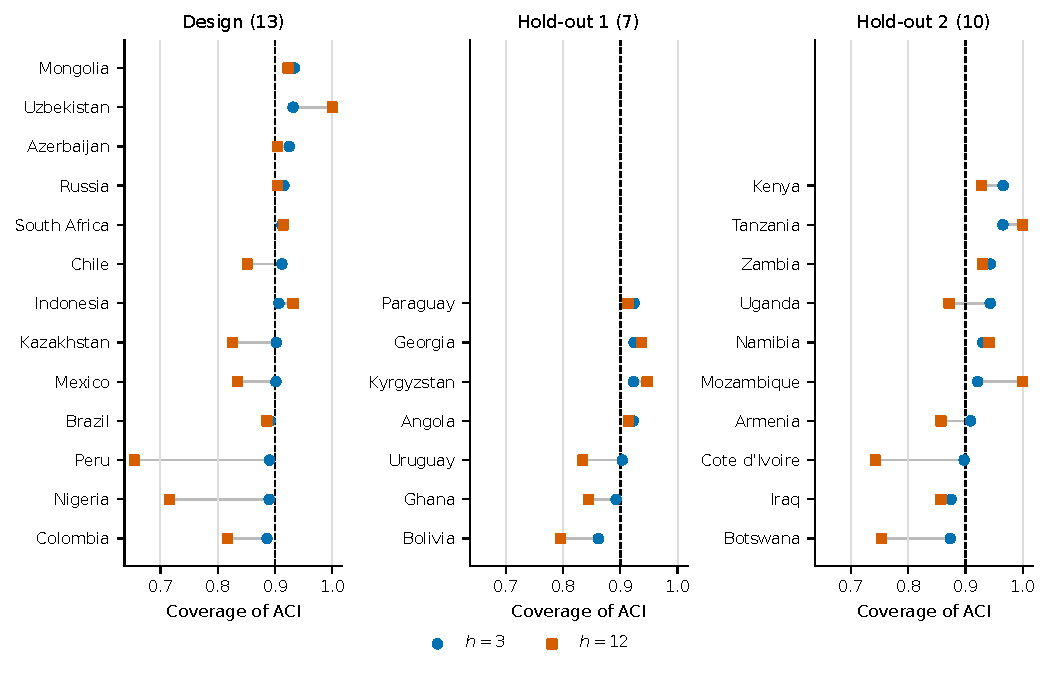
\includegraphics[width=\linewidth]{figures/fig_country_coverage.pdf}
\caption{Per-country empirical coverage of ACI, by panel, against the nominal level 0.90.}
\label{fig:country_cov}
\end{figure}

\subsection{Robustness analyses S1--S4}\label{sec:robust}

The analyses S1--S4 were written down after the hold-out result and before they were computed. They are secondary, use only existing intervals, and qualify R1--R5 without replacing them. The block length is $\max(h,12)$; S1 uses 500 bootstrap replicates and S2 and S3 use 2000.

\paragraph{S1, leave one country out (LightGBM, warm-up 48).} Table~\ref{tab:loo} shows the range of each contrast over removals and the number of removals that flip the sign of the full-sample estimate. The advantage of ACI over a calibration done once does not depend on any single country. The point estimate of ACI against rolling is negative for almost every removal, but its interval includes zero in the primary run, so ``not shown'' stands. The DRACP minus ACI estimates sit at zero and change sign when one or two countries are removed.

\begin{table}[t]
\centering
\caption{S1: range of the contrast over leave-one-country-out removals (pp of CE) and number of sign flips of the full-sample estimate.}
\label{tab:loo}
\small
\begin{tabular}{@{}lll@{}}
\toprule
Contrast, horizon & Exploratory (13 countries) & First hold-out (7 countries) \\
\midrule
ACI $-$ split, $h=3$ & $-5.1$ to $-4.2$, 0 flips & $-4.1$ to $-2.2$, 0 flips \\
ACI $-$ split, $h=6$ & $-4.1$ to $-2.5$, 0 flips & $-3.5$ to $-2.1$, 0 flips \\
ACI $-$ rolling, $h=3$ & $-2.5$ to $-1.8$, 0 flips & $-2.2$ to $-1.0$, 0 flips \\
ACI $-$ rolling, $h=6$ & $-1.7$ to $-1.3$, 0 flips & $-1.3$ to $+0.1$, 1 of 7 flips \\
DRACP $-$ ACI, $h=3$ & $0.0$ to $+0.4$, 0 flips & $-0.4$ to $-0.1$, 0 flips \\
DRACP $-$ ACI, $h=6$ & $-0.5$ to $+0.1$, 2 of 13 flips & $-0.7$ to $+0.1$, 1 of 7 flips \\
\bottomrule
\end{tabular}
\end{table}

\subsection{Width, interval score and the question of narrower intervals}\label{sec:width}

Three statistics must be kept apart when the question is whether adaptive intervals are narrower, and they do not give the same answer (Table~\ref{tab:width} and Figure~\ref{fig:width_winkler}).

\begin{table}[t]
\centering
\caption{Calibration error / Winkler ratio / median width ratio relative to rolling conformal, by panel, interval method and horizon (LightGBM, warm-up 48; a ratio below 1 is better than rolling).}
\label{tab:width}
\small
\fittable{\begin{tabular}{lcccc}
\toprule
Method & $h{=}1$ & $h{=}3$ & $h{=}6$ & $h{=}12$ \\
\midrule
\multicolumn{5}{l}{\emph{Design (13), warm-up 48}} \\
ACI & 0.013 / 0.99 / 0.91 & 0.014 / 1.06 / 0.93 & 0.035 / 1.21 / 1.11 & 0.069 / 1.00 / 1.03 \\
DRACP & 0.016 / 1.07 / 0.95 & 0.016 / 1.16 / 0.95 & 0.033 / 1.21 / 1.09 & 0.074 / 1.38 / 1.69 \\
FACI & 0.014 / 1.00 / 0.95 & 0.018 / 1.05 / 0.94 & 0.041 / 1.06 / 0.88 & 0.101 / 0.96 / 0.91 \\
Conformal PID & 0.030 / 1.00 / 0.96 & 0.033 / 1.02 / 0.98 & 0.059 / 1.02 / 0.94 & 0.105 / 1.01 / 1.01 \\
Rolling & 0.038 / 1.00 / 1.00 & 0.036 / 1.00 / 1.00 & 0.050 / 1.00 / 1.00 & 0.091 / 1.00 / 1.00 \\
Split & 0.071 / 1.08 / 1.24 & 0.060 / 1.11 / 1.29 & 0.069 / 1.02 / 1.13 & 0.139 / 0.93 / 0.94 \\
\midrule
\multicolumn{5}{l}{\emph{Hold-out 1 (7), warm-up 48}} \\
ACI & 0.020 / 0.95 / 0.84 & 0.020 / 0.99 / 0.90 & 0.025 / 1.05 / 0.88 & 0.048 / 1.12 / 1.09 \\
DRACP & 0.021 / 0.97 / 0.89 & 0.019 / 0.96 / 0.91 & 0.022 / 1.04 / 0.91 & 0.047 / 1.25 / 0.97 \\
FACI & 0.023 / 0.95 / 0.85 & 0.023 / 0.94 / 0.90 & 0.013 / 1.00 / 0.90 & 0.070 / 1.07 / 0.92 \\
Conformal PID & 0.024 / 0.98 / 0.95 & 0.028 / 0.97 / 0.95 & 0.021 / 1.00 / 0.94 & 0.079 / 1.05 / 0.99 \\
Rolling & 0.029 / 1.00 / 1.00 & 0.036 / 1.00 / 1.00 & 0.032 / 1.00 / 1.00 & 0.086 / 1.00 / 1.00 \\
Split & 0.056 / 1.11 / 1.34 & 0.050 / 1.07 / 1.23 & 0.053 / 1.06 / 1.27 & 0.119 / 1.02 / 1.09 \\
\bottomrule
\end{tabular}
}
\end{table}

\begin{figure}[t]
\centering
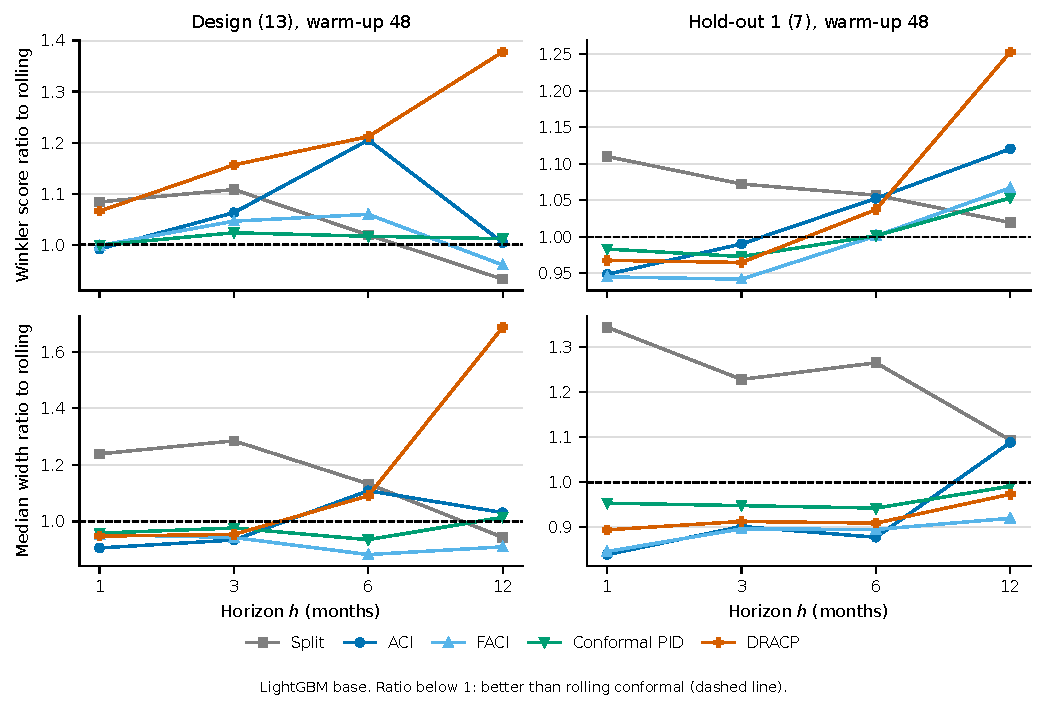
\includegraphics[width=\linewidth]{figures/fig_width_winkler.pdf}
\caption{Interval width and Winkler score of the interval methods relative to rolling conformal.}
\label{fig:width_winkler}
\end{figure}

\begin{itemize}
\item \emph{Median interval width ratio (to rolling).} At $h=1$ and $h=3$, ACI, DRACP and FACI have a median width below that of rolling in both samples: ACI 0.91 and 0.93 in the exploratory data, and 0.84 and 0.90 on the first hold-out panel.
\item \emph{Pooled mean width.} The pooled mean width of ACI at $h=3$ is larger than that of rolling in both samples: 4.28 against 3.95 in the exploratory data and 5.856 against 5.786 on the hold-out panel. This indicates heavy tails in the width of the adaptive intervals. The pooled mean width of DRACP is larger than that of ACI at $h=3$ (4.97 against 4.28) and at $h=12$ (24.3 against 15.5) in the exploratory data.
\item \emph{Winkler score.} The Winkler ratio to rolling for ACI, DRACP and FACI at $h=1$ and $h=3$ is 0.94 to 0.99 on the hold-out panel and 0.99 to 1.16 in the exploratory data (ACI 1.06 and DRACP 1.16 at $h=3$). In the exploratory data ACI's Winkler score at $h=3$ was 6.3 percent higher than rolling's (95\% interval \ci{0.3}{19.4}, unadjusted $p=0.15$). At $h=6$ and $h=12$ the Winkler ratio of ACI and DRACP is above 1 in most cells of both samples (up to 1.38).
\end{itemize}
The adaptive methods have a lower median width at short horizons, but the pooled mean width and the interval score do not show a consistent gain. No efficiency advantage is established; at long horizons the better calibration is paid for with width or interval score.

\subsection{Second hold-out panel (extension)}\label{sec:panel2}

The second hold-out panel has 10 countries with 198 months of CPI from 2010-01. At warm-up 48 there are 89 pooled calendar months at $h=3$ and 83 at $h=6$; at warm-up 96 there are 41 and 35. Four base models are used: LightGBM, ARIMA, naive B and Chronos. The Holm family has four tests per base model. Warm-up 48 is the primary run; warm-up 96 is a sensitivity run and is not promoted.

Table~\ref{tab:ce_ho2} gives the calibration error at warm-up 48. At $h=3$ and $h=6$ ACI has 0.033 and 0.045 (LightGBM), 0.034 and 0.052 (ARIMA), 0.049 and 0.052 (naive B) and 0.034 and 0.050 (Chronos); DRACP has 0.023 and 0.032, 0.019 and 0.034, 0.037 and 0.034, and 0.030 and 0.038; rolling has 0.070 and 0.080, 0.066 and 0.084, 0.090 and 0.087, and 0.067 and 0.075; split has 0.104 and 0.125, 0.098 and 0.111, 0.122 and 0.105, and 0.109 and 0.107; the native ARIMA intervals have 0.058 and 0.084. For comparison, on the first hold-out panel the calibration error of the rolling window at $h=3$ and $h=6$ is 0.036 and 0.032, against 0.066 to 0.090 and 0.075 to 0.087 here. This is a descriptive observation, and its relation to the results below was not tested.

\begin{table}[t]
\centering
\caption{Calibration error by interval method, horizon and base model, second hold-out panel (10 countries, warm-up 48).}
\label{tab:ce_ho2}
\small
\fittable{\begin{tabular}{llrrrr}
\toprule
Base model & Interval & $h{=}1$ & $h{=}3$ & $h{=}6$ & $h{=}12$ \\
\midrule
LightGBM & Split & 0.084 & 0.104 & 0.125 & 0.154 \\
 & Rolling & 0.050 & 0.070 & 0.080 & 0.089 \\
 & ACI & 0.032 & 0.033 & 0.045 & 0.072 \\
 & FACI & 0.024 & 0.027 & 0.042 & 0.079 \\
 & Conformal PID & 0.043 & 0.051 & 0.070 & 0.103 \\
 & DRACP & 0.023 & 0.023 & 0.032 & 0.078 \\
\midrule
ARIMA & Split & 0.086 & 0.098 & 0.111 & 0.136 \\
 & Rolling & 0.053 & 0.066 & 0.084 & 0.089 \\
 & ACI & 0.026 & 0.034 & 0.052 & 0.074 \\
 & FACI & 0.033 & 0.023 & 0.035 & 0.075 \\
 & Conformal PID & 0.037 & 0.047 & 0.073 & 0.105 \\
 & DRACP & 0.017 & 0.019 & 0.034 & 0.071 \\
 & Native & 0.052 & 0.058 & 0.084 & 0.132 \\
\midrule
Naive B & Split & 0.079 & 0.122 & 0.105 & 0.188 \\
 & Rolling & 0.057 & 0.090 & 0.087 & 0.110 \\
 & ACI & 0.023 & 0.049 & 0.052 & 0.089 \\
 & FACI & 0.024 & 0.049 & 0.055 & 0.082 \\
 & Conformal PID & 0.054 & 0.073 & 0.074 & 0.122 \\
 & DRACP & 0.020 & 0.037 & 0.034 & 0.087 \\
\midrule
Chronos & Split & 0.078 & 0.109 & 0.107 & 0.111 \\
 & Rolling & 0.048 & 0.067 & 0.075 & 0.078 \\
 & ACI & 0.028 & 0.034 & 0.050 & 0.062 \\
 & FACI & 0.017 & 0.031 & 0.041 & 0.088 \\
 & Conformal PID & 0.040 & 0.052 & 0.073 & 0.105 \\
 & DRACP & 0.021 & 0.030 & 0.038 & 0.082 \\
\bottomrule
\end{tabular}
}
\end{table}

Table~\ref{tab:panel2primary} gives the primary contrasts for each base model.

\begin{table}[t]
\centering
\caption{Primary contrasts, second hold-out panel, warm-up 48: $T$ in pp of CE, 95\% bootstrap interval, and Holm $p$ over the four primary tests of the base model.}
\label{tab:panel2primary}
\small
\resizebox{\linewidth}{!}{%
\begin{tabular}{@{}lllll@{}}
\toprule
Base model & ACI $-$ rolling, $h=3$ & ACI $-$ rolling, $h=6$ & DRACP $-$ ACI, $h=3$ & DRACP $-$ ACI, $h=6$ \\
\midrule
LightGBM & $-3.7$ \ci{-5.1}{-0.7}; 0.008 & $-3.5$ \ci{-4.9}{+0.5}; 0.159 & $-1.0$ \ci{-2.0}{+0.9}; 0.321 & $-1.3$ \ci{-2.7}{+2.0}; 0.337 \\
ARIMA & $-3.2$ \ci{-3.6}{-1.1}; 0.004 & $-3.1$ \ci{-3.9}{-0.5}; 0.030 & $-1.5$ \ci{-2.4}{+0.8}; 0.199 & $-1.8$ \ci{-3.4}{+0.7}; 0.199 \\
Naive B & $-4.1$ \ci{-4.9}{-1.5}; 0.004 & $-3.4$ \ci{-4.7}{-0.4}; 0.039 & $-1.2$ \ci{-2.3}{+0.9}; 0.422 & $-1.8$ \ci{-3.3}{+2.5}; 0.422 \\
Chronos & $-3.3$ \ci{-4.0}{-0.3}; 0.036 & $-2.5$ \ci{-3.6}{+0.1}; 0.088 & $-0.5$ \ci{-1.8}{+1.3}; 0.454 & $-1.2$ \ci{-2.2}{+1.3}; 0.443 \\
\bottomrule
\end{tabular}}
\end{table}

ACI minus split (secondary, unadjusted $p$, at $h=3$ and $h=6$) is $-7.0$ and $-8.0$~pp for LightGBM (0.0005, 0.0005), $-6.4$ and $-5.8$ for ARIMA (0.0005, 0.001), $-7.3$ and $-5.3$ for naive B (0.001, 0.0045) and $-7.4$ and $-5.7$ for Chronos (0.0005, 0.0005). ACI with ARIMA has a lower CE than the native ARIMA intervals (0.034 against 0.058 at $h=3$ and 0.052 against 0.084 at $h=6$); the contrast with its interval is not reported for this panel. The outcomes of the rules on this panel are as follows.

\paragraph{R1 (ACI better calibrated than split).} At warm-up 48 R1 is met for all four base models at both horizons (unadjusted $p$ at most 0.0045), by $-5.3$ to $-8.0$~pp of CE. At warm-up 96 it is not met: LightGBM (0.048) and naive B (0.032) at $h=3$ have unadjusted $p$ below 0.05, all other cells are above 0.05, and with Holm over the two horizons none is below 0.05 (0.096 and 0.064). The direction replicates, and the registered threshold is met on the second panel at warm-up 48 whereas on the first hold-out panel it was met only at warm-up 96.

\paragraph{R2 (ACI improves on rolling): the result differs from the earlier panels.} At warm-up 48 R2 is met at $h=3$ for LightGBM, ARIMA and naive B (Holm 0.008, 0.004, 0.004) and at $h=6$ for ARIMA and naive B (0.030, 0.039). For Chronos at $h=3$ the Holm $p$ is 0.036 but the minimum detectable difference is undefined, so under E5 that cell is inconclusive and is not counted as met; Chronos at $h=6$ and LightGBM at $h=6$ are not met (0.088, 0.159). On the design panel and on the first hold-out panel it was not shown, and the MDE is undefined there (inconclusive). The earlier 20 countries were re-run from 2010-01 as a secondary analysis, and R2 is not significant there: the Holm $p$-values of ACI minus rolling are 0.22 to 1.0, with the MDE undefined in every cell, so these results are inconclusive under E5 and not evidence of no effect. The results are placed side by side in Table~\ref{tab:r2panels} and are not pooled.

\begin{table}[t]
\centering
\caption{R2 across panels, warm-up 48: ACI minus rolling (pp of CE) and Holm $p$ over the four tests of the run.}
\label{tab:r2panels}
\small
\resizebox{\linewidth}{!}{%
\begin{tabular}{@{}llllp{0.34\linewidth}@{}}
\toprule
Panel and run & Base model & $h=3$ & $h=6$ & Outcome \\
\midrule
Design (13), from 2000 & LightGBM & $-2.2$; 0.090 & $-1.5$; 0.078 & Not shown (MDE undefined, inconclusive) \\
First hold-out (7), from 2000 & LightGBM & $-1.6$; 0.35 & $-0.7$; 1.0 & Not shown (MDE undefined, inconclusive) \\
Design (13), re-run from 2010 & LightGBM & $-2.1$; 0.216 & $-2.0$; 0.216 & Not met; MDE undefined in every cell: inconclusive under E5 \\
Design (13), re-run from 2010 & Chronos & $-1.9$; 0.363 & $-2.0$; 0.358 & Not met; MDE undefined in every cell: inconclusive under E5 \\
First hold-out (7), re-run from 2010 & LightGBM & $-2.4$; 0.496 & $-4.7$; 0.390 & Not met; MDE undefined in every cell: inconclusive under E5 \\
First hold-out (7), re-run from 2010 & Chronos & $-1.3$; 1.000 & $-2.0$; 0.962 & Not met; MDE undefined in every cell: inconclusive under E5 \\
Second hold-out (10), from 2010 & LightGBM & $-3.7$; 0.008 & $-3.5$; 0.159 & Met at $h=3$ \\
Second hold-out (10), from 2010 & ARIMA & $-3.2$; 0.004 & $-3.1$; 0.030 & Met at both \\
Second hold-out (10), from 2010 & Naive B & $-4.1$; 0.004 & $-3.4$; 0.039 & Met at both \\
Second hold-out (10), from 2010 & Chronos & $-3.3$; 0.036 (MDE undefined: inconclusive under E5) & $-2.5$; 0.088 & Inconclusive at $h=3$; not met at $h=6$ \\
\bottomrule
\end{tabular}}
\end{table}

Three things should be read together. First, the point estimates are negative in every row of Table~\ref{tab:r2panels}. On the second panel they ($-2.5$ to $-4.1$~pp) are generally larger than on the earlier panels ($-0.7$ to $-2.4$~pp), with one exception, LightGBM on the re-run first hold-out panel at $h=6$ ($-4.7$~pp, Holm $p=0.390$, 95\% interval \ci{-9.6}{+0.5}); so the direction does not differ between panels, but its size and its distance from the registered threshold do. Second, the conclusion that ``ACI improves on a rolling window'' is reached under the registered rule on one panel and not on the other two. The data do not say why. Candidate explanations are a shorter series (198 months from 2010), lower-income and more volatile economies, a larger share of the 198 months taken by the warm-up, and a rolling window with a larger calibration error here; none of them was tested, and none is claimed. Third, the four base models are evaluated on the same 10 countries and the same months, so the three ``met'' cells at $h=3$ are not three independent confirmations, and the Holm correction does not extend across base models. We do not average the panels into one statement and we do not select the panel on which the rule is met.

\paragraph{Warm-up 96 on the second panel shows nothing.} After a warm-up of 96 the panel has 41 pooled months at $h=3$ and 35 at $h=6$. ACI minus rolling is $-1.0$ to $-3.3$~pp at $h=3$ (Holm $p$ 0.147 to 1.0). At $h=6$ it is $+0.2$~pp (LightGBM), $+1.1$~pp (Chronos), $-0.5$~pp (ARIMA) and $-0.6$~pp (naive B), with Holm $p$ of 0.59 or more. The minimum detectable difference is undefined for every contrast. The run is a sensitivity run, it neither confirms nor contradicts the primary run, and it is not promoted.

\paragraph{R3 stays inconclusive.} At warm-up 48 DRACP has a lower CE than ACI in every cell, by 0.5 to 1.8~pp, and no difference has Holm $p$ below 0.05 (0.199 to 0.454). Equivalence within 2~pp holds only for Chronos at $h=3$ (TOST $p=0.0385$) and is not shown in the other seven cells ($p$ 0.15 to 0.76). At warm-up 96 equivalence holds for LightGBM and naive B at $h=3$ ($p=0.0375$ and 0.013) and not in the other six cells, and DRACP is better than ACI only at $h=6$ for naive B ($-2.3$~pp, Holm $p=0.002$). R3 requires the same verdict at both warm-ups, so it is not met. Under E5 every DRACP minus ACI contrast at warm-up 48 has an undefined minimum detectable difference and is inconclusive whatever its $p$-value, including the equivalence of Chronos at $h=3$. The small and consistent tendency of DRACP towards a lower CE at warm-up 48 is a descriptive observation and not a result.

\paragraph{E5, power.} At warm-up 48 the minimum detectable difference for ACI minus rolling is 3.2~pp ($h=3$) and 6.1~pp ($h=6$) for LightGBM, 3.2 and 3.5~pp for ARIMA, 1.2 and 3.5~pp for naive B, and 6.6~pp for Chronos at $h=6$; it is undefined for Chronos at $h=3$, so that cell is not conclusive under the rule even though the Holm $p$ is 0.036. Where R2 is not met (LightGBM and Chronos at $h=6$) the minimum detectable difference of 6.1 and 6.6~pp is larger than the estimates, so ``not met'' there is not evidence that the effect is absent.

\paragraph{E2, dependence on the base model.} On this panel the direction and the size of the contrasts are alike for the four base models (Tables~\ref{tab:ce_ho2} and~\ref{tab:panel2primary}). The conclusions about R1 and R3 do not depend on the base model; the conclusion about R2 at $h=6$ does (met for ARIMA and naive B, not for LightGBM and Chronos), and at $h=3$ Chronos is inconclusive under E5 while LightGBM, ARIMA and naive B are met. On the earlier 20 countries re-run from 2010-01 the effect is weaker: ACI minus rolling is $-1.3$ to $-4.7$~pp with Holm $p$ 0.22 to 1.0, and ACI minus split is $-3.5$ to $-9.4$~pp with unadjusted $p$ between 0.002 and 0.045. R4 (delayed feedback) was not part of the extension, and no instant-feedback run was made on the second panel.

\begin{figure}[t]
\centering
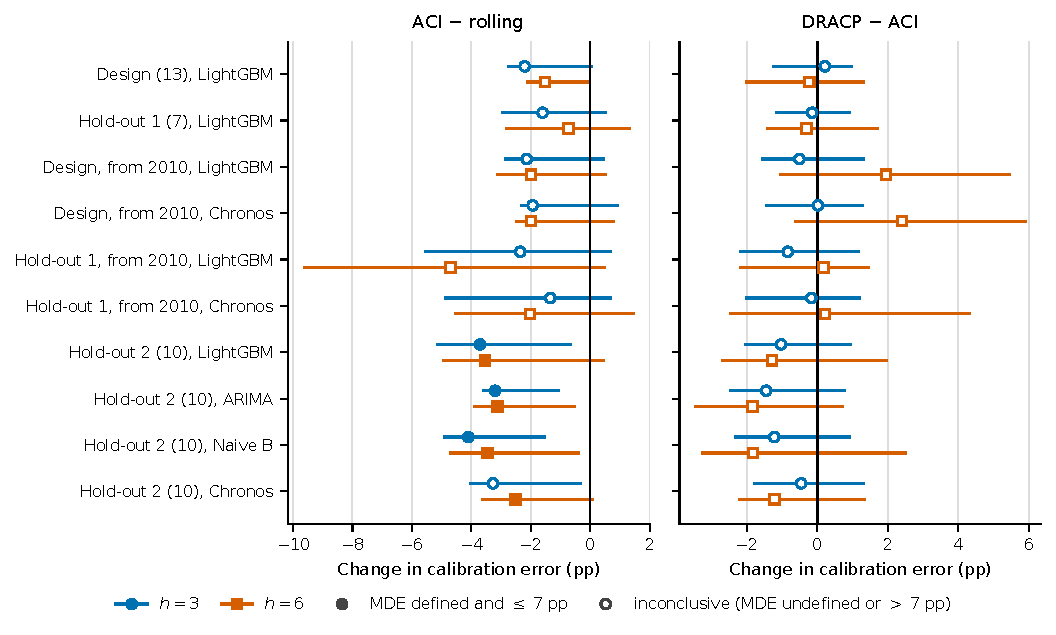
\includegraphics[width=\linewidth]{figures/fig_contrasts_forest.pdf}
\caption{Forest plot of the change in calibration error (pp) for ACI minus rolling and DRACP minus ACI, with 95\% block-bootstrap intervals. Contrasts with an undefined minimum detectable difference are inconclusive under rule E5 regardless of the interval.}
\label{fig:forest}
\end{figure}

Figure~\ref{fig:forest} shows the contrasts side by side. The figure is a display of the same estimates as in Tables~\ref{tab:contrasts},~\ref{tab:panel2primary} and~\ref{tab:r2panels}; it does not pool the panels.

\subsection{Ablation study}\label{sec:ablation}

The ablations vary one design choice at a time: the base model, the warm-up, the feedback delay, and the reference interval (native against conformal). A fifth subsection reports the point accuracy of Chronos.

\subsubsection{Base model}\label{sec:basemodel}

The contrasts were recomputed with ARIMA and naive B as base models of the conformal methods on the design and first hold-out panels (S2, Appendix Table~\ref{tab:s2full}), and Table~\ref{tab:ablation_base} gives the same ablation on the second hold-out panel with four base models. ACI minus split is negative for all three base models in both samples; for naive B at $h=6$ on the first hold-out panel it is $-10.6$~pp. All DRACP minus ACI equivalence tests at warm-up 48 say ``equivalent'' within 2~pp, except naive B at $h=6$ on the hold-out panel ($p=0.0515$); at warm-up 96 on the hold-out panel most are ``not shown''. The direction ``ACI better than rolling'' holds for every base model and both samples, but the unadjusted $p$-values range from 0.016 to 0.48, and none survives the correction of the pre-specified family. For example, at $h=3$ on the hold-out panel ACI minus rolling is $-1.6$~pp for LightGBM ($p=0.087$), $-3.0$~pp for ARIMA ($p=0.030$) and $-0.9$~pp for naive B ($p=0.22$); at $h=6$ it is $-0.7$ ($p=0.48$), $-1.6$ ($p=0.21$) and $-3.2$~pp ($p=0.053$). ARIMA and naive B give similar ACI coverage at $h=6$ in the exploratory data (0.895 and 0.908). On the second hold-out panel the base-model dependence is described in Section~\ref{sec:panel2}.

\begin{table}[t]
\centering
\caption{Ablation over the base model on the second hold-out panel (warm-up 48): relative mean absolute error (naive B $=1$, all target months including flagged months), calibration error of ACI and of rolling, and ACI minus rolling in pp of CE with Holm $p$.}
\label{tab:ablation_base}
\small
\fittable{\begin{tabular}{lrrrrrrrr}
\toprule
& \multicolumn{2}{c}{Rel. MAE} & \multicolumn{2}{c}{CE, ACI} & \multicolumn{2}{c}{CE, rolling} & \multicolumn{2}{c}{ACI $-$ rolling, pp (Holm $p$)} \\
\cmidrule(lr){2-3}\cmidrule(lr){4-5}\cmidrule(lr){6-7}\cmidrule(lr){8-9}
Base model & $h{=}3$ & $h{=}6$ & $h{=}3$ & $h{=}6$ & $h{=}3$ & $h{=}6$ & $h{=}3$ & $h{=}6$ \\
\midrule
Naive B & 1.000 & 1.000 & 0.049 & 0.052 & 0.090 & 0.087 & $-$4.1 (0.004) & $-$3.4 (0.039) \\
ARIMA & 0.602 & 0.570 & 0.034 & 0.052 & 0.066 & 0.084 & $-$3.2 (0.004) & $-$3.1 (0.030) \\
LightGBM & 0.619 & 0.593 & 0.033 & 0.045 & 0.070 & 0.080 & $-$3.7 (0.008) & $-$3.5 (0.159) \\
Chronos & 0.586 & 0.581 & 0.034 & 0.050 & 0.067 & 0.075 & $-$3.3 (0.036) & $-$2.5 (0.088) \\
\bottomrule
\end{tabular}
}
\end{table}

\subsubsection{Warm-up: 48 against 96}\label{sec:warmup}

Warm-up 96 is a sensitivity run applied to all methods; it is not promoted to the primary configuration. Table~\ref{tab:ablation_warmup} and Figure~\ref{fig:warmup} compare the two. On the first hold-out panel ACI minus split moves from $-3.0$ and $-2.8$~pp at warm-up 48 to $-4.1$ and $-5.9$~pp at warm-up 96, and this change is what turns R1 from not met to met; ACI minus rolling is $-1.6$ and $-0.7$~pp at 48 and $-1.5$ and $-1.1$~pp at 96, with Holm $p$ 0.35 and 1.0 against 0.59 and 0.99. Equivalence of DRACP and ACI is shown at warm-up 48 and not at 96 (Section~\ref{sec:holdout}). The 96-month warm-up removes target months, leaving 157 and 151 pooled months at $h=3$ and $h=6$ against 205 and 199, so the sample for the comparison is also smaller. On the second hold-out panel the warm-up of 96 leaves 41 and 35 pooled months and shows nothing (Section~\ref{sec:panel2}). The comparison between warm-ups is a sensitivity analysis and does not select a configuration.

\begin{table}[t]
\centering
\caption{Ablation over the warm-up size: calibration error of ACI and rolling, ACI minus rolling and Holm $p$ at warm-up 48 (primary) and 96 (sensitivity, not promoted), by panel.}
\label{tab:ablation_warmup}
\small
\fittable{\begin{tabular}{llcrrrrrrrr}
\toprule
\multicolumn{3}{c}{} & \multicolumn{2}{c}{CE, ACI} & \multicolumn{2}{c}{CE, rolling} & \multicolumn{2}{c}{ACI $-$ rolling (pp)} & \multicolumn{2}{c}{Holm $p$} \\
\cmidrule(lr){4-5}\cmidrule(lr){6-7}\cmidrule(lr){8-9}\cmidrule(lr){10-11}
Panel & Base & $h$ & 48 & 96 & 48 & 96 & 48 & 96 & 48 & 96 \\
\midrule
Design (13) & LightGBM & 3 & 0.014 & 0.022 & 0.036 & 0.035 & $-$2.2 & $-$1.3 & 0.090 & 0.132 \\
 &  & 6 & 0.035 & 0.039 & 0.050 & 0.054 & $-$1.5 & $-$1.5 & 0.078 & 0.132 \\
\midrule
Hold-out 1 (7) & LightGBM & 3 & 0.020 & 0.027 & 0.036 & 0.042 & $-$1.6 & $-$1.5 & 0.350 & 0.592 \\
 &  & 6 & 0.025 & 0.030 & 0.032 & 0.041 & $-$0.7 & $-$1.1 & 1.000 & 0.990 \\
\midrule
Hold-out 2 (10) & LightGBM & 3 & 0.033 & 0.045 & 0.070 & 0.058 & $-$3.7 & $-$1.3 & 0.008 & 0.278 \\
 &  & 6 & 0.045 & 0.069 & 0.080 & 0.067 & $-$3.5 & +0.2 & 0.159 & 1.000 \\
\midrule
Hold-out 2 (10) & ARIMA & 3 & 0.034 & 0.043 & 0.066 & 0.053 & $-$3.2 & $-$1.0 & 0.004 & 0.340 \\
 &  & 6 & 0.052 & 0.081 & 0.084 & 0.086 & $-$3.1 & $-$0.5 & 0.030 & 0.682 \\
\midrule
Hold-out 2 (10) & Naive B & 3 & 0.049 & 0.050 & 0.090 & 0.083 & $-$4.1 & $-$3.3 & 0.004 & 0.147 \\
 &  & 6 & 0.052 & 0.071 & 0.087 & 0.077 & $-$3.4 & $-$0.6 & 0.039 & 0.593 \\
\midrule
Hold-out 2 (10) & Chronos & 3 & 0.034 & 0.048 & 0.067 & 0.063 & $-$3.3 & $-$1.5 & 0.036 & 1.000 \\
 &  & 6 & 0.050 & 0.084 & 0.075 & 0.073 & $-$2.5 & +1.1 & 0.088 & 1.000 \\
\bottomrule
\end{tabular}
}
\end{table}

\begin{figure}[t]
\centering
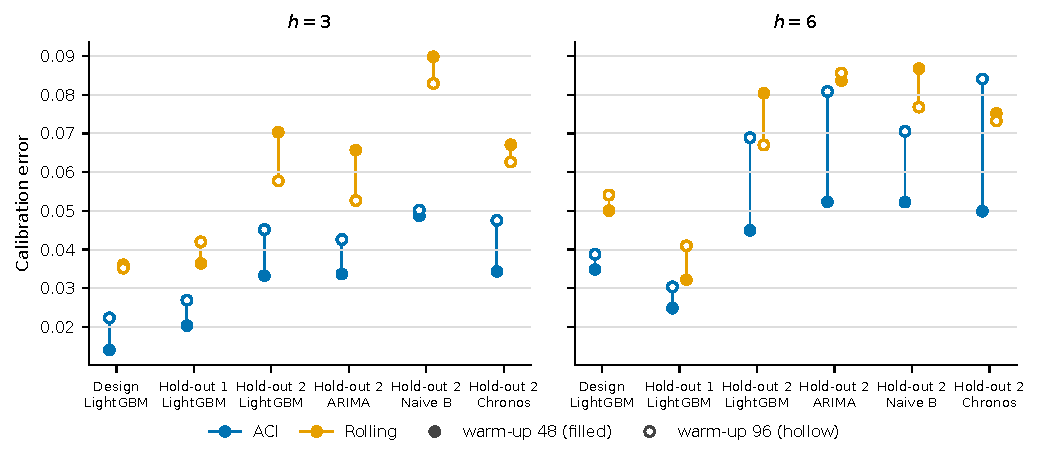
\includegraphics[width=\linewidth]{figures/fig_warmup_sensitivity.pdf}
\caption{Sensitivity of the contrasts to the warm-up size (48 against 96 residuals). Warm-up 96 is a sensitivity run and is not promoted to the primary result.}
\label{fig:warmup}
\end{figure}

\subsubsection{Feedback delay}\label{sec:feedback}

At $h=12$ pooled coverage is below nominal for every method (0.83 to 0.88 on the first hold-out panel, 0.82 to 0.87 in the exploratory data), with the qualification on the bootstrap intervals given in Section~\ref{sec:explor}. To examine the role of delayed feedback, the diagnostic run releases each outcome at origin $+1$ instead of origin $+12$. Table~\ref{tab:feedback} gives coverage with instant feedback minus coverage with delayed feedback, with a paired block-bootstrap 95 percent interval over the same (unit, origin) cells. For ACI the change is $+4.1$~pp (\ci{1.4}{7.8}) in the exploratory data (1738 cells) and $+2.4$~pp (\ci{-0.1}{4.8}) on the hold-out panel (1009 cells); for DRACP $+4.3$ (\ci{1.4}{7.5}) and $+3.9$~pp (\ci{1.6}{6.5}); for FACI $+8.3$ (\ci{4.3}{13.6}) and $+6.4$~pp (\ci{2.5}{9.6}); for conformal PID $+5.1$ and $+5.3$~pp; for rolling $+1.3$~pp in both; split conformal does not use feedback, so its difference is zero by construction.

\begin{table}[t]
\centering
\caption{Ablation over the feedback delay (S3): coverage at $h=12$ with delayed and with instant feedback, and the difference in pp with a 95\% paired block-bootstrap interval.}
\label{tab:feedback}
\small
\fittable{\begin{tabular}{lrrcrrc}
\toprule
& \multicolumn{3}{c}{Design (13), 1738 cells} & \multicolumn{3}{c}{Hold-out 1 (7), 1009 cells} \\
\cmidrule(lr){2-4}\cmidrule(lr){5-7}
Method & Delayed & Instant & Diff. (pp) [95\% CI] & Delayed & Instant & Diff. (pp) [95\% CI] \\
\midrule
Split & 0.864 & 0.864 & +0.0 [+0.0, +0.0] & 0.861 & 0.861 & +0.0 [+0.0, +0.0] \\
Rolling & 0.869 & 0.882 & +1.3 [+0.2, +3.1] & 0.872 & 0.885 & +1.3 [+0.1, +1.7] \\
ACI & 0.864 & 0.905 & +4.1 [+1.4, +7.8] & 0.884 & 0.908 & +2.4 [$-$0.1, +4.8] \\
FACI & 0.825 & 0.907 & +8.3 [+4.3, +13.6] & 0.835 & 0.900 & +6.4 [+2.5, +9.6] \\
Conformal PID & 0.837 & 0.888 & +5.1 [+2.0, +9.0] & 0.833 & 0.886 & +5.3 [+2.5, +7.9] \\
DRACP & 0.863 & 0.906 & +4.3 [+1.4, +7.5] & 0.865 & 0.904 & +3.9 [+1.6, +6.4] \\
\bottomrule
\end{tabular}
}
\end{table}

On the hold-out panel ACI coverage is 0.884 with delayed feedback and 0.908 with instant feedback. R4 as registered (ACI at least $+3$~pp) is not met: the result is $+2.4$~pp. The interval \ci{-0.1}{4.8} is compatible with no effect and with an effect of about 5~pp. For FACI and DRACP the effect is positive in both samples. The statement supported is that feedback delay accounts for part of the shortfall at $h=12$, with a size that depends on the method and the sample. It is not shown that delay is, or is not, the main cause. The diagnostic is not a valid forecasting setup and is not a primary result.

\subsubsection{Native intervals against conformal calibration}\label{sec:native}

The analysis S7 compares conformal calibration with the native (parametric) intervals of ARIMA (Gaussian) and ETS (simulated). It is post hoc (seventh protocol entry), secondary and carries no multiplicity correction; the $p$-values are unadjusted and descriptive. ETS has no conformal version in the engine, so for ETS the native calibration error is reported without a contrast. Table~\ref{tab:native} gives the mean over countries of the calibration error. In the exploratory data the native ARIMA intervals have a CE of 0.047, 0.066, 0.089 and 0.137 at $h=1,3,6,12$ against 0.010, 0.015, 0.026 and 0.079 for ARIMA with ACI, and native ETS has 0.044, 0.051, 0.064 and 0.116. On the first hold-out panel the corresponding numbers are 0.053, 0.058, 0.062 and 0.073 (native ARIMA), 0.014, 0.013, 0.024 and 0.040 (ARIMA with ACI) and 0.056, 0.035, 0.048 and 0.053 (native ETS).

\begin{table}[t]
\centering
\caption{Ablation over the reference interval (S7, post hoc): calibration error of native ARIMA and ETS intervals and of ARIMA with ACI, and the contrast ACI minus native (pp of CE, 95\% interval, unadjusted $p$).}
\label{tab:native}
\small
\fittable{\begin{tabular}{lcrrrcr}
\toprule
Panel & $h$ & ARIMA native & ARIMA + ACI & ETS native & ACI $-$ native, pp [95\% CI] & $p$ \\
\midrule
Design (13) & 1 & 0.047 & 0.010 & 0.044 & $-$3.7 [$-$4.6, $-$0.6] & 0.004 \\
 & 3 & 0.066 & 0.015 & 0.051 & $-$5.1 [$-$6.2, $-$1.0] & 0.003 \\
 & 6 & 0.089 & 0.026 & 0.064 & $-$6.4 [$-$7.7, $-$1.3] & 0.002 \\
 & 12 & 0.137 & 0.079 & 0.116 & $-$5.8 [$-$7.8, $-$1.9] & 0.003 \\
\midrule
Hold-out 1 (7) & 1 & 0.053 & 0.014 & 0.056 & $-$3.9 [$-$4.5, $-$1.3] & $<$0.001 \\
 & 3 & 0.058 & 0.013 & 0.035 & $-$4.5 [$-$4.8, $-$0.6] & 0.010 \\
 & 6 & 0.062 & 0.024 & 0.048 & $-$3.8 [$-$4.4, +1.2] & 0.082 \\
 & 12 & 0.073 & 0.040 & 0.053 & $-$3.3 [$-$4.9, +1.3] & 0.100 \\
\midrule
Hold-out 2 (10) & 1 & 0.052 & 0.026 & -- & -- & -- \\
 & 3 & 0.058 & 0.034 & -- & -- & -- \\
 & 6 & 0.084 & 0.052 & -- & -- & -- \\
 & 12 & 0.132 & 0.074 & -- & -- & -- \\
\bottomrule
\end{tabular}
}
\end{table}

The contrast ACI minus native, with ARIMA as base model, is in the exploratory data $-3.7$, $-5.1$, $-6.4$ and $-5.8$~pp at $h=1,3,6,12$ (95\% intervals \ci{-4.6}{-0.6}, \ci{-6.2}{-1.0}, \ci{-7.7}{-1.3}, \ci{-7.8}{-1.9}; unadjusted $p$ 0.004, 0.003, 0.002, 0.003) and on the first hold-out panel $-3.9$ (\ci{-4.5}{-1.3}; $p$ below 0.001), $-4.5$ (\ci{-4.8}{-0.6}; 0.010), $-3.8$ (\ci{-4.4}{+1.2}; 0.082) and $-3.3$~pp (\ci{-4.9}{+1.3}; 0.100). Conformal calibration with ACI gives a lower calibration error than the native intervals of the same ARIMA model at every horizon in both samples, by about 3 to 6~pp. On the hold-out panel the interval for the difference excludes zero at $h=1$ and $h=3$ and includes zero at $h=6$ and $h=12$. The mean coverage of the native ARIMA intervals looks acceptable on the hold-out panel (0.943, 0.930, 0.919 and 0.885 at $h=1,3,6,12$) because over-coverage in some countries offsets under-coverage in others; the calibration error shows the dispersion. The ETS native intervals have calibration errors of the same order as the ARIMA native ones in both samples. This contrast is secondary and post hoc, so the evidence against native intervals is weaker in procedure than the pre-specified contrasts, although its direction is consistent.

\subsubsection{Point accuracy of Chronos}\label{sec:chronos}

Months before 2025-01 are flagged \texttt{possibly\_seen} for Chronos, which may have met these public series in pretraining. The relative mean absolute error on the second hold-out panel over all target months, warm-up 48 (naive B $=1$; below 1 is better), is 0.737, 0.586, 0.581 and 0.934 for Chronos at $h=1,3,6,12$, against 0.779, 0.602, 0.570 and 0.880 for ARIMA and 0.817, 0.619, 0.593 and 0.943 for LightGBM. This comparison includes months on which Chronos may have an unfair advantage and is not used for any claim about Chronos; it has no intervals and no ETS, which deviates from E3 (Section~\ref{sec:extension}).

Following E4, claims about accuracy are drawn only from target months from 2025-01. These are 22 calendar months with 567 country-month cells per horizon, pooled over the 30 countries of the three panels. Table~\ref{tab:chronos_mae} gives the relative mean absolute error by horizon and model and the difference in mean absolute error (Chronos minus the other model, in pp of cumulative growth; negative favours Chronos) with a paired block-bootstrap 95\% interval (blocks of 3 months, months resampled jointly across countries); the intervals are unadjusted and descriptive. Figure~\ref{fig:chronos} displays the comparison.

\begin{table}[t]
\centering
\caption{Point accuracy of Chronos on the clean target months from 2025-01 (22 months, 30 countries): mean absolute error relative to naive B, and difference in mean absolute error with a paired block-bootstrap 95\% interval (pp; negative favours Chronos).}
\label{tab:chronos_mae}
\small
\fittable{\begin{tabular}{crrrccc}
\toprule
& \multicolumn{3}{c}{Relative MAE (naive B $=1$)} & \multicolumn{3}{c}{MAE difference, Chronos $-$ other (pp)} \\
\cmidrule(lr){2-4}\cmidrule(lr){5-7}
$h$ & Chronos & LightGBM & ARIMA & vs LightGBM & vs ARIMA & vs naive B \\
\midrule
1 & 0.774 & 0.824 & 0.854 & $-$0.023 [$-$0.047, $-$0.007] & $-$0.037 [$-$0.053, $-$0.021] & $-$0.104 [$-$0.134, $-$0.081] \\
3 & 0.699 & 0.725 & 0.773 & $-$0.031 [$-$0.078, +0.036] & $-$0.086 [$-$0.139, $-$0.031] & $-$0.350 [$-$0.519, $-$0.206] \\
6 & 0.654 & 0.694 & 0.700 & $-$0.084 [$-$0.129, $-$0.025] & $-$0.097 [$-$0.204, +0.002] & $-$0.720 [$-$0.905, $-$0.527] \\
12 & 0.895 & 0.995 & 0.905 & $-$0.245 [$-$0.465, $-$0.019] & $-$0.024 [$-$0.122, +0.139] & $-$0.256 [$-$0.449, $-$0.041] \\
\bottomrule
\end{tabular}
}
\end{table}


\begin{figure}[t]
\centering
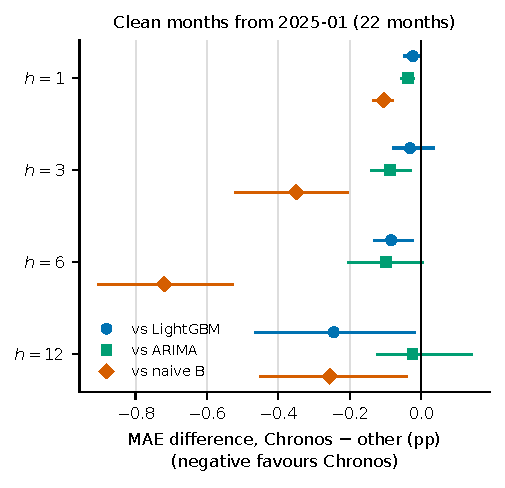
\includegraphics[width=\linewidth]{figures/fig_chronos_accuracy.pdf}
\caption{Point accuracy of Chronos relative to the other forecasters by horizon. Claims are limited to the 22 target months from 2025-01; earlier months are flagged as possibly seen in pretraining.}
\label{fig:chronos}
\end{figure}

On these clean months the relative mean absolute error of Chronos is 0.774, 0.699, 0.654 and 0.895 at $h=1,3,6,12$ (LightGBM 0.824, 0.725, 0.694, 0.995; ARIMA 0.854, 0.773, 0.700, 0.905). Against LightGBM the interval excludes zero at $h=1$, 6 and 12, and against ARIMA at $h=1$ and 3 (at $h=6$ its upper limit is $+0.002$); against naive B it excludes zero at every horizon. No interval favours LightGBM or ARIMA over Chronos. The reading is that Chronos was at least as accurate as LightGBM and ARIMA in this period and more accurate than the naive baseline. The sample is thin (22 months), the block length is short because of it, the leakage assumption (a cutoff of 2025-01) is not verified, and the results are descriptive and not a ranking of forecasters. Calibration contrasts for Chronos (Section~\ref{sec:panel2}) use all months with the flag, as specified in E4, and no calibration analysis restricted to the clean months is reported.

\subsection{Stress, post-2025-06 months and Kazakhstan}\label{sec:other}

\paragraph{Stress analysis (secondary, exploratory).} For the exploratory sample at $h=3$, coverage in the top decile of exchange-rate stress at the forecast origin is 0.849 for ACI, 0.869 for DRACP and 0.874 for split, against roughly 0.87 to 0.98 in the other deciles; at $h=6$ it is 0.864, 0.879 and 0.874. With about 200 observations per decile the standard error is roughly 2.5~pp, so the top-decile shortfall of ACI at $h=3$ is about two standard errors. The deciles in between are not monotone. The same 13 countries shaped the design, many deciles, methods and horizons were examined, and the underlying association between stress and forecast error is weak (Section~\ref{sec:shockvalid}). No stress result is reported for the hold-out panels, and no confirmatory claim about stress is made.

\paragraph{The post-2025-06 months of the 13 countries (not used).}\label{sec:confirm13} The run \texttt{confirm13} evaluates the 13 design countries on target months from 2025-07. Eleven countries contribute (Nigeria ends in 2024-12 because of the CPI break; Russia has no usable stretch after 2022-03), each with at most 16 months. With blocks of 12 months on at most 16 months the run is degenerate: confidence limits coincide with the estimate and $p$-values sit at the resampling floor. It is not used for any claim. Pooled coverage in that period is high for every method (ACI 0.904, 0.922 and 0.940 at $h=1,3,6$, from 167 unit-months), which is consistent with calmer inflation, and no conclusion is drawn.

\paragraph{Kazakhstan (post hoc, descriptive).}\label{sec:kz} The title does not name Kazakhstan because the main results contain no separate Kazakhstan analysis, but Kazakhstan was the original focus of the study, so it is reported alone. The analysis S6 is post hoc, descriptive and carries no test. Kazakhstan is one of the 13 design countries, so the numbers come from the exploratory sample and are not independent of the design. There are 137 monthly origins at $h=1$ (133, 127 and 115 at $h=3,6,12$), with target months 2014-02 to 2025-06, so the period after the August 2015 float is mixed with the preceding managed regime. The standard error of a coverage figure from about 137 correlated origins is roughly 3~pp, so only the larger gaps are clearly outside noise. ACI, DRACP and FACI stay close to 0.90 up to $h=6$ (Appendix~\ref{app:extra}), while the rolling window, conformal PID and the one-shot split calibration under-cover at short horizons (rolling 0.825 and split 0.730 at $h=1$); at $h=12$ coverage is below nominal for every method (0.713 to 0.835). The pattern is consistent with a series that changed regime in 2015, where a calibration that cannot adapt fast enough falls behind, but the data do not isolate that mechanism.

\subsection{The language-model explainer: status}

The evaluation of the explanation layer (Section~\ref{sec:platform}) has not been run on a real language model, and no result is reported. The test suite of the explanation layer has 18 tests (31 together with the 13 platform-service tests); these tests exercise the code with a deterministic fake client and are not results about a language model.
